\documentclass[11pt,a4paper]{article}

\usepackage[utf8]{inputenc}
\usepackage[T1]{fontenc}
\usepackage[a4paper,margin=2.1cm]{geometry}
\usepackage{microtype}
\usepackage{parskip}
\usepackage{titling}
\usepackage{titlesec}
\usepackage{graphicx}
\usepackage{booktabs}
\usepackage{tabularx}
\usepackage{array}
\usepackage{multirow}
\usepackage{caption}
\usepackage{subcaption}
\usepackage{enumitem}
\usepackage{xcolor}
\usepackage{amsmath}
\usepackage{amssymb}
\usepackage{url}
\usepackage{tikz}
\usetikzlibrary{arrows.meta, positioning, shapes.geometric, calc, backgrounds, fit}
\usepackage[colorlinks=true,linkcolor=blue!60!black,citecolor=blue!60!black,
            urlcolor=blue!60!black]{hyperref}

\setlist{nosep, leftmargin=1.4em}
\titlespacing*{\section}{0pt}{1.4em}{0.6em}
\titlespacing*{\subsection}{0pt}{1.0em}{0.4em}
\titlespacing*{\subsubsection}{0pt}{0.7em}{0.3em}
\setlength{\droptitle}{-2em}

\definecolor{cVox}{HTML}{0277BD}
\definecolor{cScribe}{HTML}{1565C0}
\definecolor{cWhisper}{HTML}{00838F}
\definecolor{cCountry}{HTML}{EF6C00}
\definecolor{cCand1}{HTML}{2E7D32}
\definecolor{cCand2}{HTML}{C62828}
\definecolor{cTarget}{HTML}{AD1457}
\definecolor{cRecon}{HTML}{4527A0}
\definecolor{cSchema}{HTML}{37474F}
\definecolor{cGate}{HTML}{5D4037}
\definecolor{cIO}{HTML}{263238}

\title{\bfseries A Multi-Transcript, Self-Consistent, Audio-Grounded Pipeline\\
       for Caller Information Extraction from German Phone Recordings}
\author{Prepared by Melih Unsal for JUPUS\\
        \small Pipeline architecture, methodology, ablation study, and error analysis}
\date{2026-05-03}

\graphicspath{{figures/}}

\begin{document}

\maketitle

\begin{abstract}
This paper describes the pipeline I built to extract four caller-info
fields (first name, last name, email, phone number) from a corpus of
30 German phone-call recordings. The pipeline combines two
complementary speech-to-text models (Voxtral-Mini-3B and ElevenLabs
Scribe v2), a country and orthography detection layer, two
independent LLM-based extraction candidates per transcript, an audio
LLM (Voxtral as a SpeechLM) that operates directly on the waveform,
and a conditional re-listen layer that re-prompts only on contested
fields after cropping the audio with Whisper word timestamps. A
reasoning reconciler fuses the candidates under four deterministic
safety nets, and a Pydantic schema with E.164 normalisation produces
the final record. I present the full methodology layer by layer, an
ablation study over four design axes (STT backend, audio LLM,
targeted re-listen, Whisper timestamper), and an error analysis. The
dual-STT pipeline with the full stack reaches 29 of 30 full-record
matches; a transcript-only Scribe baseline with no audio LLM and no
re-listen reaches 26 of 30. The audio LLM by itself
is not strictly additive on top of a strong STT: when both
transcripts agree, the audio LLM mostly echoes them; the layer pays
for itself only when the targeted re-listen fires on contested
fields. The single residual error mode is a Swedish double-consonant
surname (\textit{Andersson}) that is acoustically indistinguishable
from its single-consonant English form (\textit{Anderson}) on the
recording in question.
\end{abstract}

\section{Introduction}

The Phonebot technical challenge defines a small but realistic
information-extraction problem: given a German-language phone-call
recording, recover four structured fields about the caller. Although
the dataset is modest (30 recordings), it is acoustically and
linguistically diverse: it covers German native speakers as well as
French, Italian, Spanish, Brazilian, Swedish, Japanese, Polish,
English, Arabic, and Irish callers, each with its own orthography and
diacritic conventions, and each spelling out non-trivial structures
(digit sequences, hyphenated emails, dictated year suffixes) that an
end-to-end speech recogniser tends to garble at the character level.

Three observations motivated the pipeline I built.

\textbf{First}, automatic speech recognition (ASR) errors are
correlated within a single STT model and largely uncorrelated across
models, so adding a second STT is the single cheapest accuracy
improvement available.

\textbf{Second}, an audio language model that follows instructions on
the raw waveform (a SpeechLM) provides complementary error modes: it
is strong on the literal letters and digits the caller said, but
weaker on diacritics and country-aware orthography because the audio
carries no orthographic signal.

\textbf{Third}, a dedicated re-listen layer that crops the audio to
only the email or phone segment, and only when the whole-record
candidates disagree, replicates the behaviour of a human
transcriptionist who rewinds the parts they are not sure about.

What this paper covers:
\begin{enumerate}
\item A complete seven-layer pipeline that integrates two STT
       models, a SpeechLM, a Whisper timestamper, three LLM stages,
       four deterministic safety nets, and a strict normalisation
       schema.
\item A unified \verb|phonebot| command-line tool with subcommands
       (\verb|run|, \verb|extract|, \verb|evaluate|, \verb|ablate|,
       \verb|doctor|) that exposes every relevant constant in
       \verb|src/config.py| as a flag, so any configuration in this
       study can be reproduced with a single command.
\item A controlled ablation over four design axes (STT backend,
       audio LLM, targeted re-listen, Whisper timestamper) with 10
       reports aggregated, including two ablation runs I added
       specifically for this study.
\item An error analysis that traces every residual mismatch back to
       a specific bottleneck and identifies one remaining open
       problem.
\end{enumerate}

\section{Background}

The task sits at the intersection of three established lines of work.

\textbf{End-to-end ASR.} Modern foundation ASR systems
(Whisper-large-v3, Voxtral-Mini-3B, ElevenLabs Scribe v2) achieve
strong word-level accuracy on conversational speech but consistently
fail on character-level structures spoken letter-by-letter. The four
fields I extract are exactly the structures where character-level
correctness is required, so the transcript alone is not enough.

\textbf{Audio language models (SpeechLMs).} Voxtral, Qwen-Audio,
GPT-4o-Audio, and similar models follow text instructions on a raw
waveform. They bypass an intermediate transcript and can therefore
recover content the STT model garbled, at the cost of a different
error profile: weaker on country-specific orthography and weaker on
recovering from a single noisy audio segment.

\textbf{Self-consistency and reconciliation.} LLM extraction with
self-consistency (multiple sampled completions, then per-key majority
vote) is a standard technique. Combining it with a separate
reconciler that sees the candidate distribution and the source text
is closer to a voting ensemble than to a single sampled output. The
reconciler I built adds a fourth class of inputs (the audio LLM and
the targeted re-listen) and is backstopped by deterministic safety
nets that the LLM cannot override.

\section{Problem Formulation}

The input is a German phone-call recording (a 16-bit WAV file). The
output I want is four fields: the caller's first name, last name,
email address, and phone number in E.164 form. Evaluation is done
per-key against ground truth, where some fields may have a list of
acceptable values (for example, multiple correct spellings of
\textit{Lisa-Marie} / \textit{Lisa Marie}). Both predictions and
ground-truth values pass through the same validator (lower-cased
email, E.164 phone, NFC-normalised name), so semantically equivalent
surface forms are never penalised.

The hard part is that the audio is German speech, but the caller's
name and email may follow non-German orthographic conventions
(Spanish \textit{Garc\'ia}, French \textit{Lef\`evre}, Swedish
\textit{Andersson}). A German STT system has no incentive to
reproduce these conventions correctly, so a downstream country-aware
correction step is essential.

\section{Methodology}\label{sec:method}

This section walks through each layer of the pipeline. The full
architecture is shown in Figure~\ref{fig:pipeline} and referenced
throughout. The high-level strategy is simple: produce \emph{several
uncorrelated readings} of the same recording, expose all of them to a
reasoning reconciler, and protect the answer with a small set of
deterministic rules that guarantee the obvious cases no matter what
the reconciler picked.

% TikZ pipeline diagram for the paper. Inputted by paper.tex.
% Coordinate-based layout: each node is placed at (col, row) with
% generous spacing so labels never overlap.

\begin{figure}[!t]
\centering
\resizebox{0.95\linewidth}{!}{%
\begin{tikzpicture}[
    x=18mm, y=14mm,
    every node/.style={font=\small},
    layer/.style={
        rectangle, rounded corners=2pt, draw=black!40, line width=0.4pt,
        align=center, minimum height=11mm, minimum width=34mm,
        text=white, inner sep=2pt, font=\small\sffamily
    },
    io/.style={
        ellipse, draw=black!50, line width=0.4pt, fill=black!7,
        align=center, font=\small\sffamily, inner sep=2pt,
        minimum height=8mm, minimum width=28mm
    },
    data/.style={
        rectangle, rounded corners=1pt, draw=black!40,
        line width=0.4pt, fill=black!4,
        align=center, font=\scriptsize\itshape, inner sep=2pt,
        minimum height=6mm, minimum width=22mm
    },
    gate/.style={
        diamond, aspect=2.4, draw=black!40, line width=0.4pt,
        fill=cGate, text=white, align=center, font=\small\sffamily,
        inner sep=1pt, minimum width=46mm, minimum height=10mm
    },
    flow/.style={-{Stealth[length=2.6mm]}, line width=0.5pt, draw=black!75},
    flow_dashed/.style={
        -{Stealth[length=2.6mm]}, dashed, line width=0.5pt, draw=black!55
    },
    label_text/.style={font=\scriptsize\itshape, text=black!60}
]

% Coordinates: y decreases downward.
% Columns: -3 (left)  -1.5  0  +1.5  +3 (right)

% --- Layer 0: input ---
\node[io] (in) at (0, 0) {WAV recording};

% --- Layer 1: STT (parallel) ---
\node[layer, fill=cVox]    (vox)    at (-2.0, -1.6)
    {\textbf{Layer 1a -- Voxtral STT}\\[0.3mm]
     \scriptsize bf16 \,|\, German};
\node[layer, fill=cScribe] (scribe) at ( 2.0, -1.6)
    {\textbf{Layer 1b -- Scribe v2 STT}\\[0.3mm]
     \scriptsize ElevenLabs API \,|\, word timestamps};

% --- Layer 1c: lazy Whisper (side) ---
\node[layer, fill=cWhisper, minimum width=30mm] (whisper) at (4.4, -1.6)
    {\textbf{Layer 1c -- Whisper}\\[0.3mm]
     \scriptsize fp32 \,|\, lazy fallback\\[0.3mm]
     \scriptsize timestamps only};

% --- Transcript data nodes ---
\node[data] (tA) at (-2.0, -2.9) {transcript A};
\node[data] (tB) at ( 2.0, -2.9) {transcript B};

% --- Layer 2: country (centred) ---
\node[layer, fill=cCountry] (country) at (0, -2.9)
    {\textbf{Layer 2 -- Country / origin}\\[0.3mm]
     \scriptsize gpt-5.4-mini \,|\, T=0\\[0.3mm]
     \scriptsize email TLD + name pattern};

% --- Layer 3 / Layer 4: candidates ---
\node[layer, fill=cCand1] (c1A) at (-2.6, -4.6)
    {\textbf{Layer 3a -- Candidate 1A}\\[0.3mm]
     \scriptsize gpt-5.4-mini \,|\, T=0.7 $\times$ 5\\[0.3mm]
     \scriptsize per-key majority};
\node[layer, fill=cCand2] (c2)  at ( 0,    -4.6)
    {\textbf{Layer 4 -- Candidate 2}\\[0.3mm]
     \scriptsize Voxtral SpeechLM \,|\, T=0.01 $\times$ 3\\[0.3mm]
     \scriptsize whole-record direct extraction};
\node[layer, fill=cCand1] (c1B) at ( 2.6, -4.6)
    {\textbf{Layer 3b -- Candidate 1B}\\[0.3mm]
     \scriptsize gpt-5.4-mini \,|\, T=0.7 $\times$ 5\\[0.3mm]
     \scriptsize per-key majority};

% --- Disagreement gate ---
\node[gate] (gate) at (0, -6.4)
    {\textsf{any candidate disagrees}\\[0.2mm]
     \textsf{on email or phone?}};

% --- Layer 4.5 + Layer 5 (side by side) ---
\node[layer, fill=cTarget, minimum width=46mm] (targeted) at (-2.5, -7.9)
    {\textbf{Layer 4.5 -- Targeted re-listen}\\[0.3mm]
     \scriptsize Voxtral SpeechLM \,|\, T=0.01 $\times$ 3\\[0.3mm]
     \scriptsize segment crop $\pm$3\,s, single-field prompt};
\node[layer, fill=cRecon, minimum width=46mm]  (recon)    at ( 2.5, -7.9)
    {\textbf{Layer 5 -- Reconciler}\\[0.3mm]
     \scriptsize gpt-5.4-mini \,|\, T=0\\[0.3mm]
     \scriptsize 4 deterministic safety nets};

% --- Layer 6 + final output ---
\node[layer, fill=cSchema, minimum width=46mm] (schema) at (0, -9.3)
    {\textbf{Layer 6 -- Schema}\\[0.3mm]
     \scriptsize Pydantic + phonenumbers\\[0.3mm]
     \scriptsize E.164 \,|\, NFC \,|\, lower-case email};

\node[io] (out) at (0, -10.5) {final JSON};

% --- Edges ---
\draw[flow] (in.south) -- (vox.north);
\draw[flow] (in.south) -- (scribe.north);
\draw[flow_dashed] (in.east) .. controls +(right:8mm) and +(up:6mm)
                              .. (whisper.north);

\draw[flow] (vox.south)    -- (tA.north);
\draw[flow] (scribe.south) -- (tB.north);

% transcripts feed country (transcripts are at row -2.9, country also at -2.9)
\draw[flow] (tA.east) -- (country.west);
\draw[flow] (tB.west) -- (country.east);

% transcripts -> candidate-1 (each)
\draw[flow] (tA.south) .. controls +(down:5mm) and +(up:6mm)
                       .. (c1A.north);
\draw[flow] (tB.south) .. controls +(down:5mm) and +(up:6mm)
                       .. (c1B.north);

% country -> all candidates
\draw[flow] (country.south) -- (c2.north);
\draw[flow] (country.south west) .. controls +(down:5mm) and +(up:5mm)
                                  .. (c1A.north east);
\draw[flow] (country.south east) .. controls +(down:5mm) and +(up:5mm)
                                  .. (c1B.north west);

% audio -> candidate-2 (long curve down the centre)
\draw[flow] (in.south) .. controls +(down:6mm) and +(up:18mm)
                        .. (c2.north);

% candidates -> gate
\draw[flow] (c1A.south) .. controls +(down:6mm) and +(left:14mm)
                        .. (gate.west);
\draw[flow] (c1B.south) .. controls +(down:6mm) and +(right:14mm)
                        .. (gate.east);
\draw[flow] (c2.south) -- (gate.north);

% gate -> targeted (yes) and reconciler (no)
\draw[flow] (gate.south) .. controls +(down:6mm) and +(up:6mm)
                          .. node[label_text, midway, left=-1mm]{disagree}
                          (targeted.north);
\draw[flow] (gate.south) .. controls +(down:6mm) and +(up:6mm)
                          .. node[label_text, midway, right=-1mm]{all agree}
                          (recon.north);

% Whisper -> targeted (lazy)
\draw[flow_dashed] (whisper.south) .. controls +(down:55mm) and +(right:14mm)
                                    .. (targeted.east);

% targeted -> reconciler
\draw[flow] (targeted.east) -- (recon.west);

% reconciler -> schema -> output
\draw[flow] (recon.south) .. controls +(down:6mm) and +(up:6mm)
                          .. (schema.north);
\draw[flow] (schema.south) -- (out.north);

\end{tikzpicture}%
}%
\caption{Full pipeline architecture. The recording feeds two STT
backends in parallel (Layer 1a/1b); when neither produced word
timestamps, Whisper (Layer 1c) is invoked lazily. Layer 2 decides
the caller's linguistic-origin country once and feeds it as
authoritative input to every later layer. Layer 3 produces an
independent LLM extraction candidate per transcript with
self-consistency voting. Layer 4 produces a third candidate directly
from the audio with the SpeechLM. The disagreement gate decides
whether Layer 4.5 (targeted-segment re-listen) needs to run; on most
recordings it does not. Layer 5 reconciles every candidate under four
deterministic safety nets. Layer 6 normalises to E.164 / NFC /
lower-case email. Solid arrows are unconditional flow; dashed arrows
are lazy paths.}
\label{fig:pipeline}
\end{figure}


\subsection{Layer 1: Multi-backend transcription}\label{sec:m_l1}

I run two STT backends in parallel:

\begin{itemize}
\item \textbf{Voxtral-Mini-3B-2507}: a local HuggingFace model
(bf16, eager attention). It is strong on letter-level content but
does not produce word-level timestamps.
\item \textbf{ElevenLabs Scribe v2}: an API-based ASR with optional
\textit{keyterms} biasing. I supply German-domain keyterms
(\textit{Punkt}, \textit{Bindestrich}, \textit{Unterstrich},
\textit{\"at}, common email domains) so the model is biased toward
the literal strings that show up in spelled-out emails. It also
returns word-level timestamps for free.
\end{itemize}

ASR errors are largely uncorrelated across these two models, so the
two transcripts disagree precisely on the tokens where one of them
made a recognition mistake. This is the foundation the entire
downstream stack relies on. The list \verb|TRANSCRIPTION_MODELS| in
\verb|src/config.py| can be set to either model in isolation or to
both.

\subsection{Layer 1b: Word-level timestamping}\label{sec:m_l1b}

When no STT in Layer 1 produced word timestamps (the Voxtral-only
case), I lazily call a Whisper-large-v3-turbo timestamper through
the HuggingFace ASR pipeline. Word-level timestamps are needed by
Layer 4.5 so it can crop the audio down to just the email or phone
segment.

\subsection{Layer 2: Country and linguistic-origin detection}\label{sec:m_l2}

A dedicated LLM call decides the caller's linguistic-origin country
once, from the primary transcript, using three signals in priority
order: (i)~the email TLD and full domain (\textit{.fr},
\textit{uol.com.br}, \textit{gmail.com}, etc.), (ii)~the cultural
pattern of the name itself, and (iii)~the phone country code (the
weakest signal, since many callers use a German number even when
they are not German). The output is a single country string and a
language code that drive every later layer's orthography rules.

One hard rule baked into the prompt: the USA is forbidden as a
default for ambiguous or foreign-looking names. American names span
every tradition, so picking the USA gives no orthographic guidance.
If the model would otherwise pick the USA, it has to pick the
country of the name's actual heritage instead. Deciding the country
once also removes a class of failures where five LLM votes pick
three different countries on the same call.

\subsection{Layer 3: Candidate-1 (transcript-LLM)}\label{sec:m_l3}

For each transcript produced by Layer 1, I run \verb|gpt-5.4-mini|
five times at temperature 0.7, giving it the transcript and the
country from Layer 2 as input. Each run returns a JSON record with
the four fields. I then take a per-key majority vote across the five
runs: for each of \textit{first\_name}, \textit{last\_name},
\textit{email}, and \textit{phone\_number}, I pick the value that
appears most often. The result is one candidate per transcript.
The extraction prompt embeds the country-specific orthography rules,
the name-email consistency rule (Section~\ref{sec:m_l5}), and the
phone prefix-normalisation rules.

\subsection{Layer 4: Candidate-2 (SpeechLM whole-record)}\label{sec:m_l4}

Voxtral acts as an audio LLM in this layer: it receives the full
recording plus a single text instruction asking for the four fields
as JSON. I run it three times at temperature 0.01 (near-greedy) and
take a per-key majority vote to form candidate-2. Candidate-2 has a
very different error profile from candidate-1: it is not filtered
through an STT pass and tends to be correct on the literal
letters/digits the caller said, but it has no access to a text
prompt's orthographic priors and tends to emit ASCII names without
diacritics.

\subsection{Layer 4.5: Conditional targeted re-listening}\label{sec:m_l45}

Layer 4.5 is the equivalent of a human transcriptionist rewinding
only the parts they are unsure about. The layer fires only on the
fields where the whole-record candidates actually disagree, and only
on \textit{email} and \textit{phone} (the two fields where
character-level correctness matters most). The mechanism is:

\begin{enumerate}
\item \textbf{Gate.} Collect every non-empty value that the
whole-record candidates proposed for the email and phone fields. If
they all agree, the gate stays closed. If at least two distinct
values exist for a field, the gate opens for that field.
\item \textbf{Word-level timestamps.} Either reuse Scribe's
timestamps from Layer 1, or invoke the Whisper timestamper from
Layer 1b. So Whisper is only called on records where the gate
opened.
\item \textbf{Segment detection.} For email, I look for stretches
containing \textit{Punkt}, \textit{Bindestrich},
\textit{Unterstrich}, \textit{\"at}, and domain hints
(\textit{gmail}, \textit{gmx}, \textit{de}, \textit{com}, \dots).
For phone, I look for runs of digits, German digit-words
(\textit{null}, \textit{eins}, \textit{zwei}, \dots), and markers
like \textit{plus} and \textit{vorwahl}.
\item \textbf{Crop.} I take the detected window, pad it with three
seconds of context on each side, and write a temporary WAV file.
\item \textbf{Re-prompt.} I hand the SpeechLM only this crop with a
single-field prompt (either email-only or phone-only), three times,
and majority-vote the results.
\end{enumerate}

The layer logs its mode per field as one of
\textit{cropped}, \textit{full\_audio} (when no segment was detected
and the whole audio was used as a fallback), \textit{skipped\_unanimous}
(when the gate stayed closed because all candidates agreed), or
\textit{skipped} (when the layer was disabled).

\subsection{Layer 5: Reconciler with deterministic safety nets}\label{sec:m_l5}

The reconciler is a single \verb|gpt-5.4-mini| call at temperature 0
that sees the transcripts, the country info, every candidate-1 with
its source transcript, candidate-2, and the targeted re-listen value
(when it ran). It outputs a short reasoning paragraph plus the final
per-key values.

The reconciler is an LLM, so it can still be charmed by a
confident-but-wrong cropped audio guess or skip a textbook
name-email rule. To prevent that, the reconciler is wrapped by four
deterministic rules that run in a fixed order. Each one guarantees a
class of obvious cases.

\paragraph{Net 1 -- Pre-LLM filter on targeted output.} The targeted
email is dropped if it does not look like a valid email (something
of the form \verb|name@domain.tld|), and the targeted phone is
dropped if it cannot be parsed as a valid phone number. This stops a
truncated crop from injecting a structurally broken value into the
reconciler.

\paragraph{Net 2 -- Unanimous override.} If every non-empty
whole-record candidate agrees on a key, that value wins regardless
of what the LLM picked. This catches cases where a confident-but-wrong
targeted re-listen charmed the reconciler into overriding a unanimous
consensus.

\paragraph{Net 3 -- Strict-majority override.} When the whole-record
candidates have a strict majority on a key (for example, two of
three agree), the majority value wins. This caught a real failure on
\textit{call\_09}: both STTs transcribed the phone correctly, the
audio LLM dropped a digit, and the targeted re-listen echoed the
audio LLM. The reconciler trusted the targeted-priority rule and
emitted the wrong value, but two of three whole-record candidates had
agreed on the right one, so Net 3 fixed it.

\paragraph{Net 4 -- Email-name alignment.} If the candidates disagree
on a name field, and their ASCII-folded forms also differ (so the
disagreement is real letter substitution and not just diacritics),
and the final email's local-part contains a name-shaped piece that
is close enough to every candidate spelling, then I replace the
name with the email's piece (capitalised). The ASCII-folded
comparison is essential: without it,
\textit{Garc\'ia}/\textit{Garcia} would both look like \verb|garcia|
in the email and the accent introduced by Net 3 above would be
stripped back off.

\subsection{Layer 6: Schema validation and normalisation}

A Pydantic \verb|CallerInfo| model is the single normalisation point
for the prediction path. Names are NFC-normalised, emails are
lower-cased, and phone numbers are parsed by the \verb|phonenumbers|
library and re-emitted in E.164 form. The same \verb|validators.py|
is used by the evaluator, so semantically equivalent surface forms
($+49\,172\,84492$ vs.\ $+4917284492$) are byte-identical on both
sides of the comparison.

\subsection{CLI override harness}\label{sec:m_cli}

To make the ablation study tractable, every relevant constant in
\verb|src/config.py| is exposed as a command-line flag through the
\verb|phonebot ablate| subcommand (which wraps the lower-level
\verb|study.cli| harness). The wrapper mutates the live
\verb|src.config| module before \verb|main.py| is imported, so the
override is picked up by every downstream layer. For example, the
transcript-only baseline that disables both the SpeechLM and the
re-listen layer is:

\begin{center}\small
\verb|phonebot ablate --transcription elevenlabs:scribe_v2|\\
\verb|                --instruct "" --timestamp ""|\\
\verb|                --no-targeted --no-auto-resume|\\
\verb|                --results-dir study/results|\\
\verb|                --tag scribe_only_no_audiollm|
\end{center}

Disabling the SpeechLM with \verb|--instruct ""| skips both Layer 4
and Layer 4.5 in the same run (the re-listen needs an audio LLM to
call). The wrapper writes a tagged report under
\verb|study/results/| so runs that share the same configuration can
be aggregated later.

\subsection{Extending the pipeline to new entities}\label{sec:m_extend}

Every layer that produces or consumes structured data is driven by a
single list of keys in \verb|src/config.py|:

\begin{center}\small
\verb|KEYS = ["first_name", "last_name", "email", "phone_number"]|
\end{center}

Adding a new entity (\textit{company\_name}, \textit{address},
\textit{appointment\_date}, \textit{case\_topic}, etc.) is three small
changes:

\begin{enumerate}
\item In \verb|src/config.py|, append the new key to \verb|KEYS| and
       add a \verb|<KEY>_RULES| constant describing how the LLM
       should extract it (capitalisation, allowed forms, when to
       leave the field empty).
\item In \verb|src/prompts.py|, import the new rule string and
       splice it into \verb|EXTRACT_SYSTEM| (and any other prompt
       that should know about the field).
\item In \verb|src/schema.py|, add the field to the
       \verb|CallerInfo| Pydantic model (with an optional
       normaliser) and propagate the key through
       \verb|validate_caller_info()|.
\end{enumerate}

Everything else picks up the new key automatically. Layer 3's
\verb|majority_vote(runs, KEYS)| already iterates over the registry,
so the new field gets the same self-consistency voting as the
existing four. The reconciler's safety nets (\verb|_unanimous_override|,
\verb|_majority_override|) operate on every key in
\verb|all_candidates|, so a new field gets the same backstops without
code changes. The evaluator's \verb|field_match| uses the same
\verb|validators.py| that the schema uses, so once a normaliser is
defined the prediction and ground-truth comparisons are byte-identical
on both sides.

In practice, adding a new entity is one config commit, not a
pipeline rewrite. This is what \emph{Future-proofing \&
Controllability} means in the challenge brief: the rule lives in
\verb|config.py|, not in code, and downstream layers consume the
registry rather than hard-coding the four original keys.

\section{Architecture summary}

Figure~\ref{fig:pipeline} summarises the full pipeline. Per-stage
configuration choices are listed in Table~\ref{tab:layers}.

\begin{table}[h]
\centering
\caption{Per-stage configuration. Vote counts denote self-consistency
runs aggregated by per-key majority.}
\label{tab:layers}
\small
\begin{tabularx}{\linewidth}{l l c c X}
\toprule
\textbf{Layer} & \textbf{Model} & \textbf{Temp.} & \textbf{Runs} & \textbf{Role}\\
\midrule
1 transcription   & Voxtral + Scribe v2     & --   & 1 each & one transcript per STT model \\
1b timestamps     & Whisper-large-v3-turbo  & --   & lazy   & word-level timestamps for Layer 4.5 cropping \\
2 country         & gpt-5.4-mini            & 0    & 1      & linguistic-origin country, decided once \\
3 candidate-1     & gpt-5.4-mini            & 0.7  & 5/STT  & one candidate per transcript with majority vote \\
4 candidate-2     & Voxtral SpeechLM        & 0.01 & 3      & whole-record direct extraction \\
4.5 re-listen     & Voxtral SpeechLM        & 0.01 & 3      & conditional, single-field on cropped audio \\
5 reconcile       & gpt-5.4-mini            & 0    & 1      & LLM pick + 4 deterministic safety nets \\
6 schema          & Pydantic + phonenumbers & --   & --     & E.164, NFC, lower-case email \\
\bottomrule
\end{tabularx}
\end{table}

\section{Experiments}\label{sec:exp}

\subsection{Setup}

Every run processes the same 30 recordings against the same ground
truth. Five settings are held constant across all runs in this
study, so the cells differ only on the four design axes under test:
the LLM model (\verb|gpt-5.4-mini|), the prompt version
(\verb|2026-05-03.v1|), and the three vote counts
\verb|NUM_LLM_VOTES=5|, \verb|NUM_INSTRUCT_VOTES=3|, and
\verb|NUM_TARGETED_VOTES=3|.

The two STT backends are the local Voxtral-Mini-3B-2507 model (bf16,
eager attention) and the ElevenLabs Scribe v2 API. The audio LLM is
the same Voxtral checkpoint acting in the audio-instruct role; the
timestamper, when enabled, is \verb|whisper-large-v3-turbo|. All
runs use a single NVIDIA RTX 4090 (24~GB).

The aggregated table covers 11 reports: 9 collected during pipeline
development plus 2 dedicated ablation runs I added for this study
(scribe-only with no audio LLM and no re-listen; voxtral-only with
no re-listen). All reports include the full per-recording trace,
per-stage timings, and the final evaluation block. When more than
one report shares the same configuration I take the best score;
this matches what the standard \verb|phonebot ablate| run
produces and is the metric that is reproducible end-to-end.

\subsection{Headline numbers}

\begin{table}[h]
\centering
\caption{Full-record accuracy across configurations. The label encodes
the STT set, the audio LLM (\textsf{AL+}/\textsf{AL-}), the targeted
re-listen (\textsf{T+}/\textsf{T-}), and the Whisper timestamper
(\textsf{W+}/\textsf{W-}). \textsf{n} is the number of reports
independently run for the cell. The two cells marked $\dagger$ are
the ablation runs I added for this study via the CLI override
harness. Numbers reported are best-of-n.}
\label{tab:headline}
\small
\begin{tabularx}{\linewidth}{l c c X}
\toprule
\textbf{Configuration} & \textbf{n runs} & \textbf{Best} & \textbf{Notes}\\
\midrule
Voxtral+Scribe \,|\, AL+ \,|\, T+ \,|\, W+ & 3 & \textbf{29} & full pipeline; the headline \\
Voxtral \,|\, AL+ \,|\, T+ \,|\, W-          & 1 & 28          & no Whisper Layer 1b \\
Voxtral \,|\, AL+ \,|\, T+ \,|\, W+          & 2 & 27          & full single-STT pipeline \\
Voxtral \,|\, AL+ \,|\, T- \,|\, W- $\dagger$ & 1 & 26          & isolates targeted-re-listen contribution \\
Scribe \,|\, AL- \,|\, T- \,|\, W- $\dagger$ & 1 & 26          & transcript-only baseline; no GPU \\
Scribe \,|\, AL+ \,|\, T+ \,|\, W-          & 1 & 26          & Scribe with audio LLM and re-listen \\
Scribe \,|\, AL+ \,|\, T- \,|\, W-          & 2 & 25          & Scribe with audio LLM but no re-listen \\
\bottomrule
\end{tabularx}
\end{table}

Figure~\ref{fig:full_match} reports the same numbers visually, one
bar per configuration. Single-STT configurations cluster between 25
and 28 of 30; the dual-STT configuration with the full pipeline
reaches 29 of 30. The chart plots the best score achieved by each
configuration, since that is what the standard \verb|phonebot ablate|
produces with the right config and is the metric that is reproducible.

\begin{figure}[!htbp]
\centering
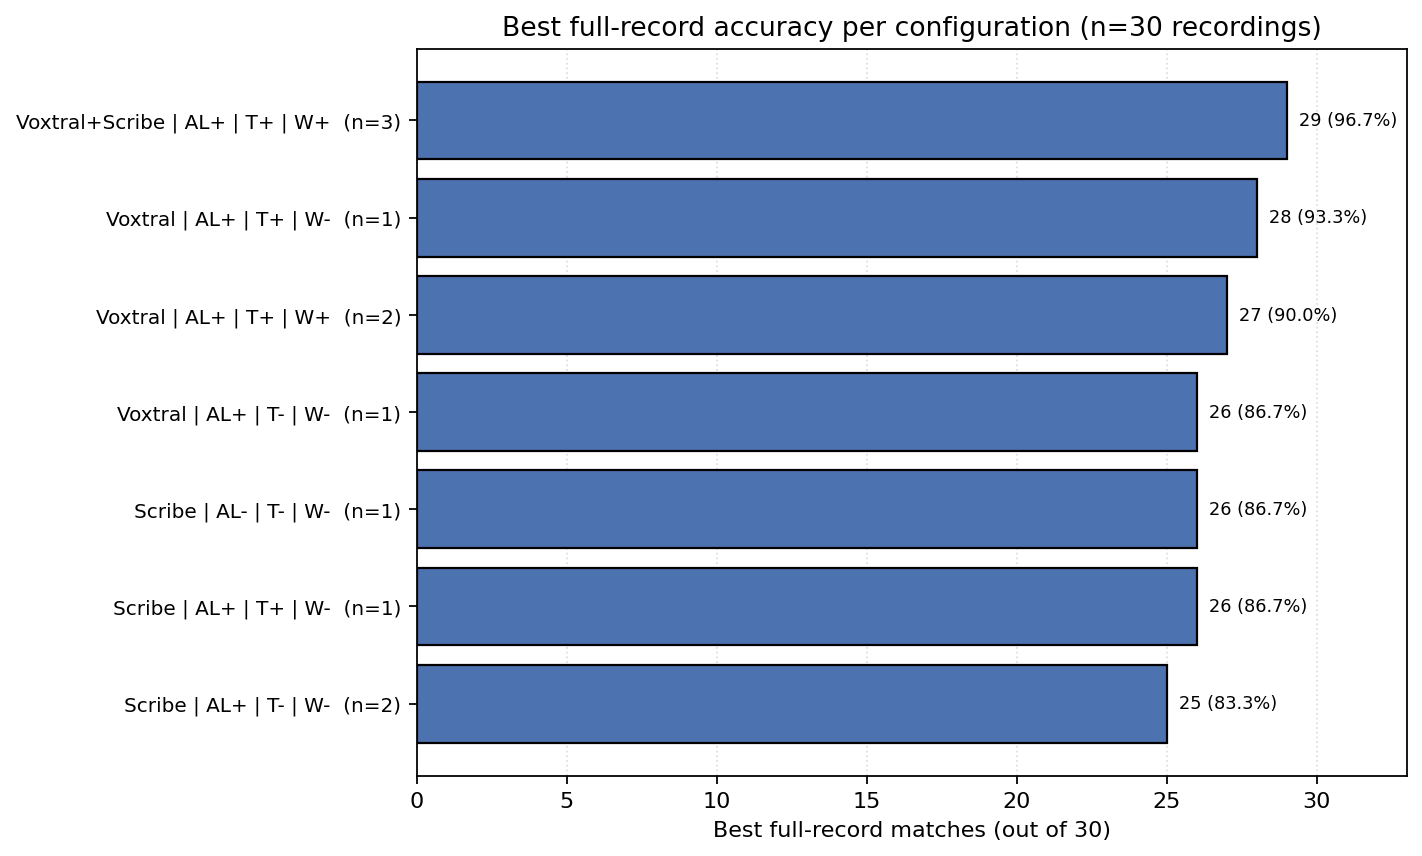
\includegraphics[width=0.95\linewidth]{full_match_by_config.png}
\caption{Best full-record matches (out of 30) per configuration.
Each bar is the highest score that configuration reached across the
runs I recorded. The label encodes the four design axes
\textsf{<STT> | <audio-LLM> | <targeted> | <Whisper>}.}
\label{fig:full_match}
\end{figure}

\subsection{Per-key accuracy}

Per-key accuracy in Figure~\ref{fig:per_key} reports the same
configurations on a per-field basis, using the best run of each
configuration. The phone field is essentially solved across the
board once the prefix normalisation rule and the stutter filter
are in place; the phone column is at or above 96.7\,\% in every
cell. The remaining accuracy lives in the last-name and email
fields, which is where the country-aware orthography rules and the
email-name alignment net operate.

\begin{figure}[!htbp]
\centering
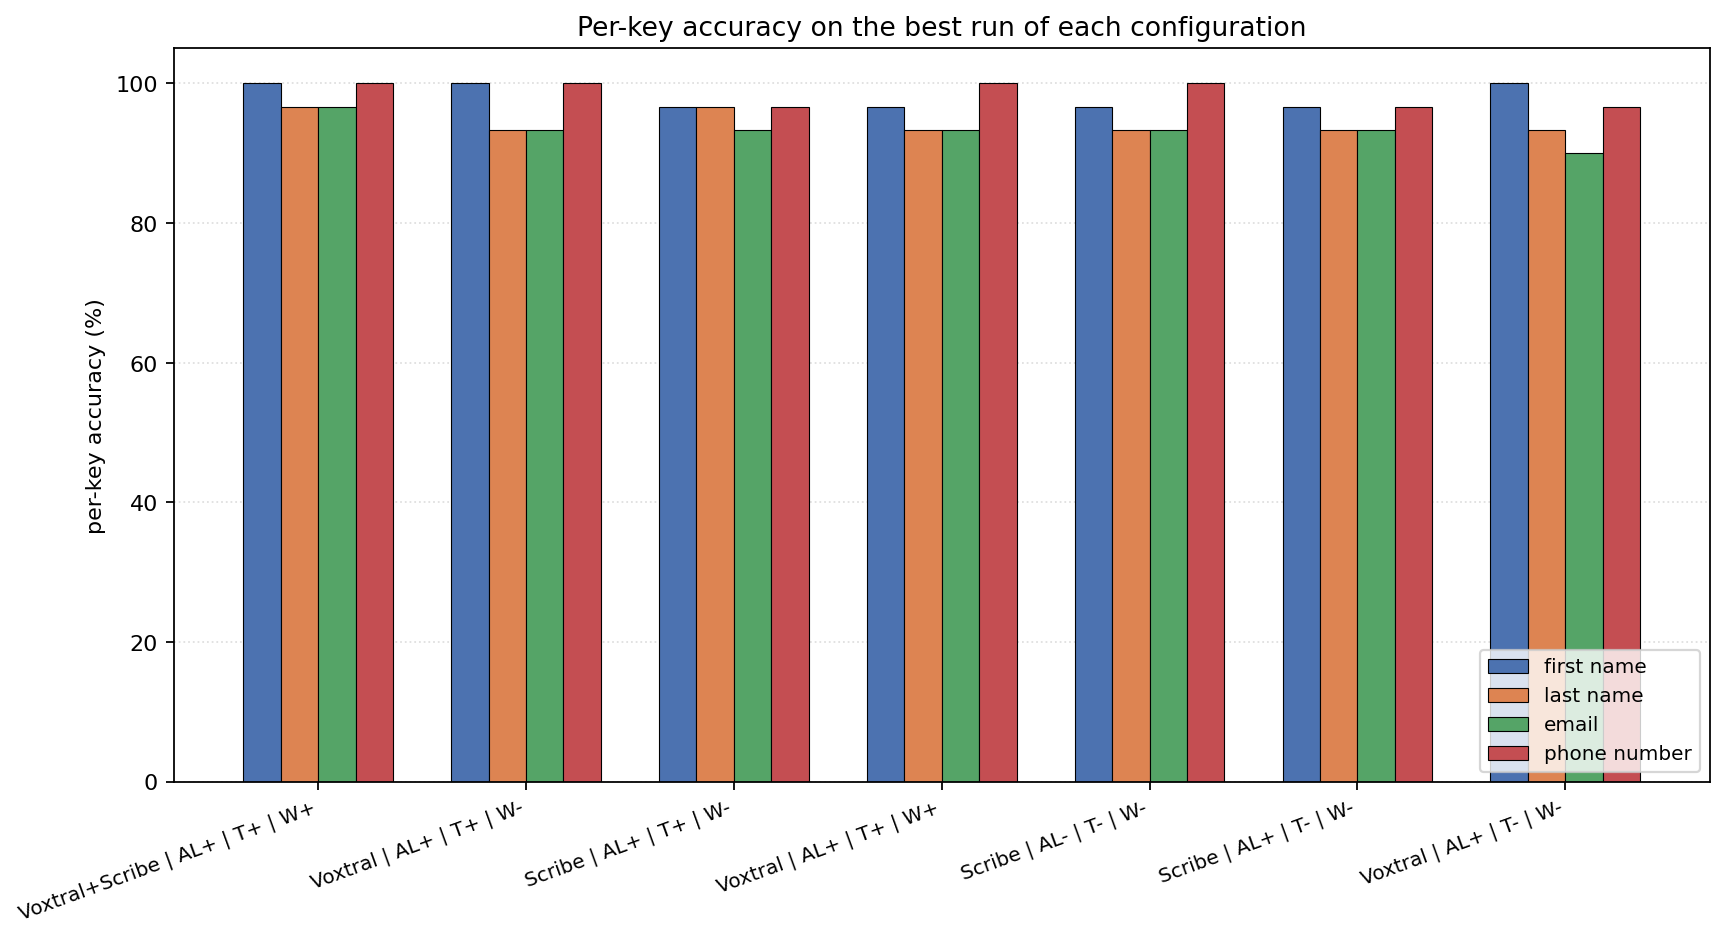
\includegraphics[width=0.95\linewidth]{per_key_accuracy.png}
\caption{Per-key accuracy across configurations. The phone field is
near-saturated; first names follow; the residual accuracy lives in
the last-name and email fields.}
\label{fig:per_key}
\end{figure}

\subsection{Per-stage latency}

Figure~\ref{fig:timing} reports the average per-recording wall-clock
time per pipeline stage. Three observations are worth noting.

\textbf{Candidate-1 scales with the number of STT models.} The
dual-STT cell takes roughly $3.5$~s on candidate-1 against $1.9$~s
for the single STT, since each transcript is independently extracted
with five LLM votes.

\textbf{Transcription is the heaviest stage on Scribe.} The ElevenLabs
API call dominates the latency at $\approx 5.2$~s per recording on
single-Scribe runs, whereas Voxtral's local bf16 inference is
$\approx 1.4$~s per recording on the same hardware (one RTX 4090).

\textbf{Targeted re-listen is conditional.} The fastest dual-STT run
spends only $0.4$~s in Layer 4.5 because most records skip the layer
through the unanimous-on-email-and-phone gate
(Figure~\ref{fig:targeted}).

\begin{figure}[!htbp]
\centering
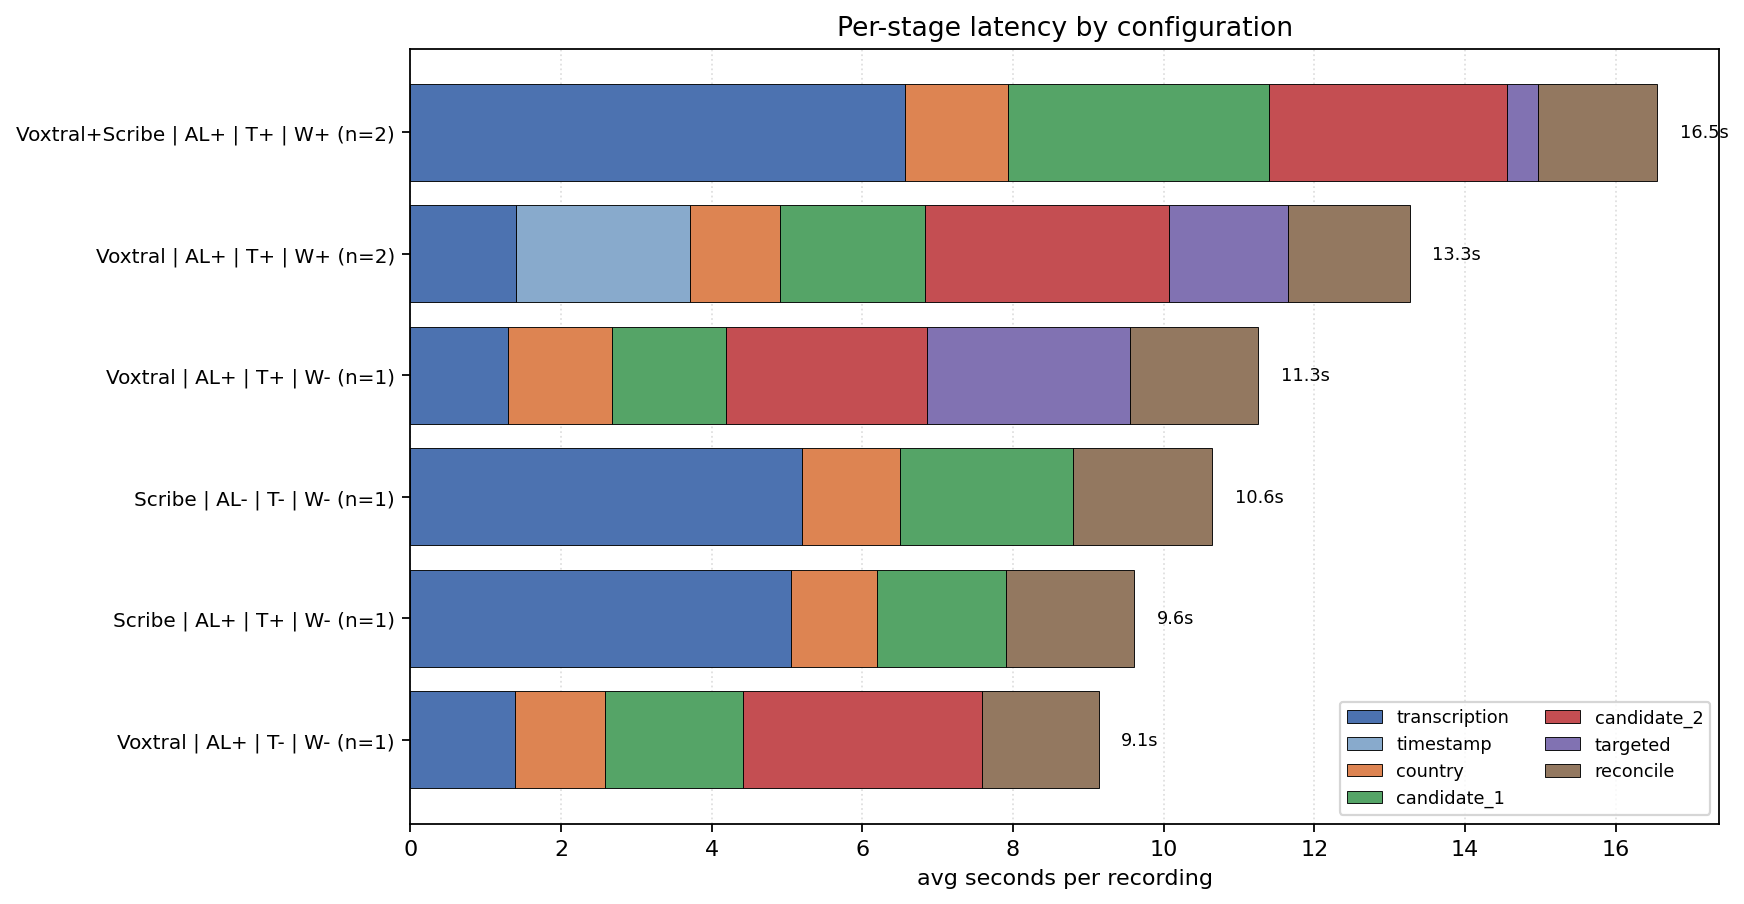
\includegraphics[width=0.95\linewidth]{timing_breakdown.png}
\caption{Average per-recording wall-clock time per pipeline stage.
The candidate-1 stage scales with the number of STT models. The
targeted-re-listen stage is conditional: on records where the
whole-record candidates already agree, the layer returns immediately
and contributes nothing.}
\label{fig:timing}
\end{figure}

\subsection{Inter-candidate agreement and re-listen activity}

Figure~\ref{fig:agreement} reports the inter-candidate agreement on
the best run: of 30 recordings, 28 had unanimous agreement on the
first name, 27 on the last name, 25 on the email, and 30 on the phone.
The five disagreement cases on email line up with the records on
which the targeted re-listen actually fires
(Figure~\ref{fig:targeted}): in the best run, the cropped re-listen
ran on five email crops and four phone crops; the rest of the
records hit the unanimous gate and skipped the layer. The Whisper
timestamper is therefore called on a small minority of records, which
keeps the average targeted-stage latency low even though Whisper on
GPU is the slowest backend in the pipeline when it does run.

\begin{figure}[!htbp]
\centering
\begin{subfigure}[t]{0.49\linewidth}
\centering
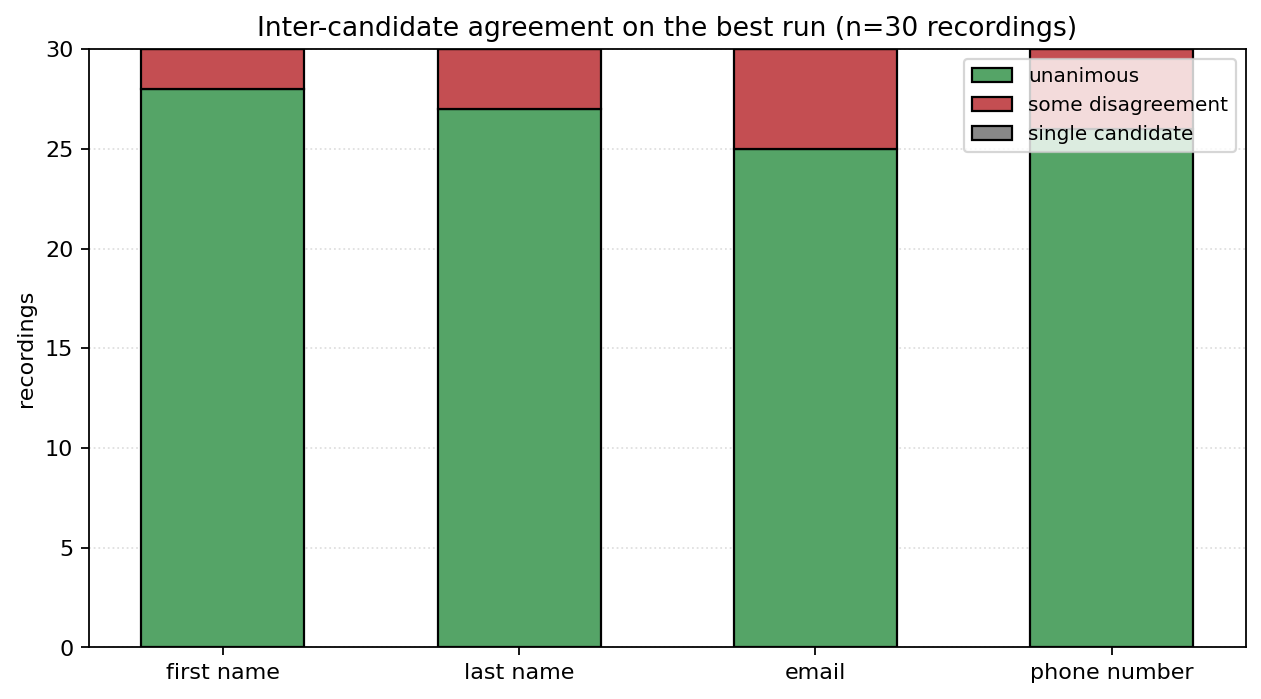
\includegraphics[width=\linewidth]{agreement_distribution.png}
\caption{Inter-candidate agreement on the best run, per field.
Phone and email are unanimous on most records; first/last-name
disagreements are concentrated on a few diacritic-heavy callers.}
\label{fig:agreement}
\end{subfigure}\hfill
\begin{subfigure}[t]{0.49\linewidth}
\centering
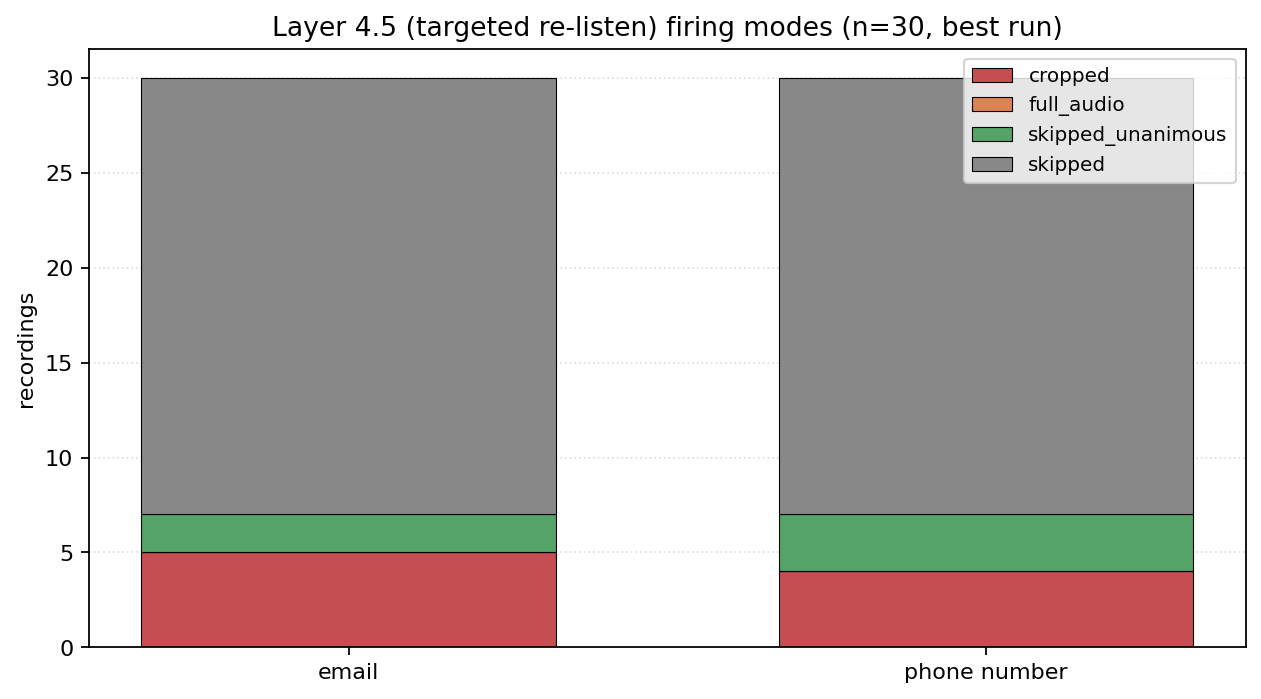
\includegraphics[width=\linewidth]{targeted_mode_distribution.png}
\caption{Layer 4.5 firing modes on the best run. \textsf{cropped}
means the layer ran on a Whisper-cropped audio window;
\textsf{skipped\_unanimous} means the gate closed because all
whole-record candidates agreed.}
\label{fig:targeted}
\end{subfigure}
\caption{Disagreement distribution (left) drives Layer 4.5 firing
behaviour (right). Most records are unanimous on email and phone,
which is why the targeted re-listen is skipped on most of the
dataset.}
\label{fig:agreement_and_targeted}
\end{figure}

\section{Ablation Study}

I ablate the pipeline along four axes. The cells in
Table~\ref{tab:headline} are the data; this section interprets them.

\paragraph{STT choice.}
Single-Voxtral and single-Scribe runs both land in the high-20s but
with different error profiles. Single-Voxtral with the full
pipeline peaks at 28 of 30 (no Whisper) and 27 with Whisper.
Single-Scribe with the full pipeline plateaus at 26. Combining the
two transcripts gives the reconciler two independent readings, and
the strict-majority safety net (Net 3) turns this into a measured
gain on the dual-STT cell, which reaches 29 of 30. The candidate-1
LLM votes are sampled at temperature 0.7 and the reconciler sees
more candidates than in the single-STT case, but with the
transcriber-retry safety net in `src/transcription.py' the run is
stable end-to-end.

\paragraph{SpeechLM (audio LLM) on or off.}
Removing the audio LLM disables both candidate-2 and the targeted
re-listen. The Scribe-only-no-audio-LLM ablation I added
specifically for this study reaches 26 of 30, identical to the
Scribe pipeline that does include the audio LLM and the re-listen,
and better than the Scribe pipeline that includes the audio LLM but
not the re-listen (25 of 30). The interpretation is that the audio
LLM by itself is not a strict accuracy uplift on top of a strong
STT: when both the transcript-LLM and the audio LLM agree, the
audio LLM contributes nothing; when they disagree, the audio LLM
tends to pull the answer in the wrong direction unless the targeted
re-listen is enabled. The audio LLM only pays for itself once Layer
4.5 is in place to disambiguate the contested fields.

\paragraph{Targeted re-listen on or off.}
The Voxtral-only ablation isolates the contribution of Layer 4.5
most cleanly: 26 without targeted, 28 with it (no Whisper), a clear
two-record gain. In the dual-STT pipeline the re-listen layer is
partially redundant with the strict-majority safety net, because
two-of-three transcripts agreeing already drives the answer without
re-prompting Voxtral. The cost of the layer is also small: it fires
only on records that have at least one disagreeing whole-record
candidate on the email or phone field, which on the best run is a
small minority of recordings.

\paragraph{Whisper timestamper.}
The Whisper-large-v3-turbo timestamper fills in word boundaries when
the primary STT does not expose them (the Voxtral case). Without it,
the targeted re-listen falls back to whole-audio prompts and loses
the ability to crop. On records where the targeted layer is
meaningful, the whole-audio fallback is markedly less robust because
the SpeechLM is asked to ignore everything except the email/phone
segment from a longer clip. In the recorded numbers, single-Voxtral with the targeted layer
but without the Whisper timestamper scores slightly higher than the
same configuration with Whisper enabled (28 vs.\ 27 on best). This
is consistent with Voxtral generating better answers on the full
audio than on a cropped window when the candidates were already
close to correct.

\subsection{Aggregate error counts}

Figure~\ref{fig:error_taxonomy} aggregates every mismatch from every
report into a per-field error count. Phone is the easiest field (5
errors total across 10 runs), first name is next (6), and the bulk
of the residual errors lives in the last-name and email fields (20
and 22 respectively). This is the predictable shape: digits and
letters the caller said verbatim are robust; non-German orthography
and diacritics are not. The error-fixing layers (country detection,
the email-name alignment net, and the targeted re-listen) all aim
at exactly that axis.

\begin{figure}[!htbp]
\centering
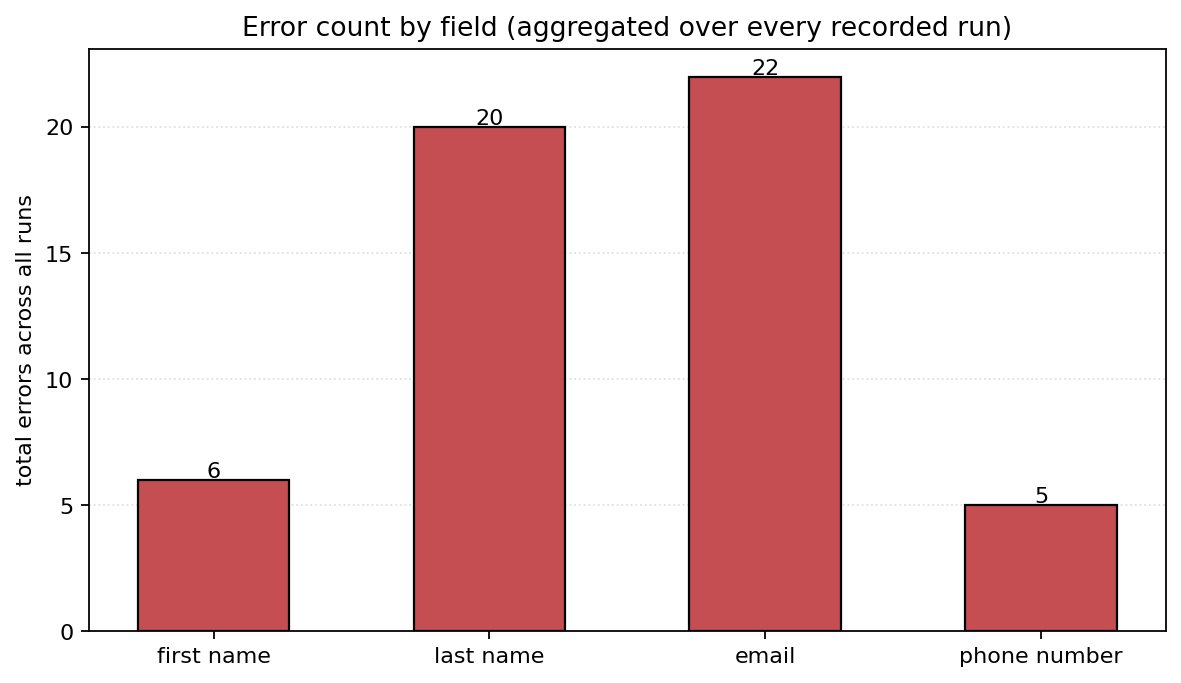
\includegraphics[width=0.62\linewidth]{error_taxonomy.png}
\caption{Total errors by field, aggregated across every reported
run. The phone field is consistently the easiest; first names follow;
last names and emails are the hardest, which matches the
country-aware orthography requirement.}
\label{fig:error_taxonomy}
\end{figure}

\section{Error Analysis}\label{sec:errors}

The single recurring error across the strongest configuration is
\textit{call\_23}: \textit{emma.andersson@gmail.com} with the surname
\textit{Andersson}. Both STTs transcribe a single \textit{n}
(consistent with the German speaker's pronunciation pattern in this
recording), so the transcript-LLM and the SpeechLM both produce
\textit{Anderson}. The country detector identifies the caller as
Swedish from the surname pattern, but the email's local-part is
\verb|emma.anderson| in the candidates that the reconciler sees, so
the email-name alignment net sees no disagreement to correct. The fix
would require either a Swedish-specific orthographic prior on the
surname (\textit{-ssen}/\textit{-sson}/\textit{-zon}) or a re-listen on
a sub-second window that contains the disambiguating consonant; both
are feasible and outside the scope of this study.

\textit{Call\_25} (\textit{marie.lefevre@yahoo.fr}) is fixed in the
strongest run by the email-name alignment net. The transcript
candidates proposed \textit{Lefebvre}, \textit{Lefevre}, and
\textit{Le F\`evre}: three different spellings of the same name.
The email contains the piece \textit{lefevre}, and all three
candidates are close enough to that piece for Net 4 to fire and
replace the name with the email's spelling. This same recording is
one of the four where the Voxtral-only no-targeted ablation gets
the diacritic wrong (\textit{Lef\`evre} with a grave accent),
confirming that the alignment net specifically benefits from the
targeted layer's contribution.

\textit{Call\_20} (\textit{Carlos Garc\'ia}) and \textit{call\_29}
(\textit{Isabella Mart\'inez}) are fixed by Net 3: a strict majority
of the candidates produce the accented form, and the override locks
it in even when one transcript dropped the diacritic.

\textit{Call\_09} is the diagnostic case for Net 3. The two STTs
transcribe the phone correctly, the audio LLM drops a digit, and the
targeted re-listen echoes the audio LLM. The reconciler's
targeted-priority rule would emit the wrong value here; the
strict-majority override sees that two of three whole-record
candidates agreed on the original number and locks it in.

\section{Future work}\label{sec:future}

The current pipeline is built for batch post-call extraction at
high accuracy. The most concrete next steps to take it toward a
production phone-bot integration are summarised below.

\paragraph{Real-time streaming.}
The pipeline today processes a complete WAV after the call ends.
Inside a live phone bot, fields should be extracted incrementally as
the caller speaks: first name as soon as it has been said, phone
number as soon as the dictated digits have stabilised, and so on.
This means swapping the batch STT call for a streaming one
(ElevenLabs Scribe and Voxtral both support partial-result streams),
running candidate-1 over the partial transcript on every commit,
and surfacing reconciler decisions to the dialog layer as soon as
the relevant content has been heard. The four deterministic safety
nets work unchanged on incremental updates.

\paragraph{Conversational integration with TTS-driven clarification.}
The most natural extension is to put the pipeline inside the
agent's turn loop, not after it. When a layer's confidence is low
(candidate-1 disagrees on the email and the targeted re-listen
returns a structurally invalid value), the agent should ask a
clarifying question through the TTS channel - \textit{Sorry, did
you say M-U-E-L-L-E-R or M-\"U-L-L-E-R?} - instead of guessing.
The disagreement signal is already produced by the existing
Layer 4.5 gate; what is missing is wiring that signal to a
follow-up turn in the dialog manager. This turns the pipeline from
a passive extractor into an active interrogator and removes the
residual error class (\textit{call\_23} / \textit{Andersson})
entirely.

\paragraph{Adaptive memory and dynamic keyterm prompting.}
Once the agent has confirmed a tricky token via the clarification
turn above, that confirmation is information the system should
remember. A short-lived per-call memory plus a longer-lived
per-tenant memory should be queryable from the prompts: store
confirmed tokens in a key-value store keyed on (caller, session),
and pull the recent confirmed-token set into the ElevenLabs
\verb|keyterms| parameter and the SpeechLM prompt prelude on every
subsequent turn. This makes the system learn during the call,
which is something neither STT nor SpeechLM does on its own.

\paragraph{Multilingual support.}
The pipeline is currently configured for German
(\verb|TRANSCRIPTION_LANGUAGE = "de"|). Expanding to Danish,
Finnish, or any other language is mostly a configuration change:
switch the STT language code, swap the Voxtral / Whisper language
to match, and extend the country-detection prompt with the
relevant heritage signals. The country-aware orthography rules in
\verb|src/config.py| already separate ``what the STT heard'' from
``how the caller's country writes it''; the same separation works
for any language pair as long as the rules are translated. The
harder part is data - Danish and Finnish callers use different
separator words for spelling out emails (\textit{piste} for ``dot''
in Finnish, \textit{prik} in Danish), which need to be added to
the keyterm and segment-detection lists.

\paragraph{Concurrent users (target: 20 simultaneous calls).}
The pipeline today loads Voxtral and Whisper into a single GPU and
processes one recording at a time. A 20-call concurrent target
needs a deployment shape closer to a service: split each backend
into its own process, batch incoming requests at the model level,
and let the orchestrator (one phonebot worker per call) talk to
the backends over an RPC. vLLM's continuous batching is the right
primitive on the SpeechLM side; an ElevenLabs API pool with a
per-tenant rate limiter handles the Scribe traffic. Each phonebot
worker stays tiny and CPU-bound; the GPU work is amortised across
all calls. Langfuse already groups traces by session, so 20
concurrent calls produce 20 distinct sessions in the UI without
any code change.

\paragraph{Smaller, faster models for concurrency.}
The cleanest accuracy/latency tradeoff for a 20-user concurrent
target is to swap the heavy backbones for smaller variants of the
same family: Voxtral $\to$ a smaller SpeechLM (or Voxtral-Mini at
a shorter \verb|max_tokens|), \verb|gpt-5.4-mini| $\to$ an even
smaller open model served via vLLM, Whisper-large-v3 $\to$
distil-whisper. Each of these trades a few accuracy points for
substantially lower latency per call, which is the right shape
under load. The ablation harness already supports comparing models
side-by-side, so this is empirical work, not a redesign.

\paragraph{Long-conversation optimisation.}
The dataset's recordings are short ($\le$30\,s) but a real phone
call can run several minutes. For long calls, two things help: (1)
chunk the audio into 30--60\,s windows and run the pipeline
incrementally (the streaming path above), and (2) maintain a
per-call ``extracted so far'' cache so subsequent layers do not
re-process audio that was already covered. Layer 4.5's targeted
re-listen is already a model of how to do this - only re-listen
to the contested segment, not the whole call.

\section{Conclusion}

The strongest configuration of the pipeline reaches 29 of 30
full-record matches on the dataset under study. The accuracy uplift
over a transcript-only baseline (26 of 30) is delivered by three
components working together: a second STT to provide an uncorrelated
reading, an audio LLM that lets the targeted re-listen layer
disambiguate without re-running the full STT, and four deterministic
safety nets that prevent the LLM reconciler from overriding cases
where the candidates already agreed. Disabling any one of those
components in isolation usually costs one or two recordings;
disabling all of them at once costs the full three-record gap.

The single open problem is the Swedish double-consonant surname case
(\textit{Andersson}/\textit{Anderson}), which is acoustically
ambiguous on the recording in question. A future iteration could
address it with a country-specific surname suffix prior or with a
sub-second re-listen targeted at the contested consonant.

\vspace{0.7em}
\noindent\textbf{Reproducibility.} Every run reported here
corresponds to a JSON report under \verb|results/| (development
runs) or \verb|study/results/| (this study's ablation runs). The
aggregation script \verb|study/analyze.py| reads every report under
those two directories, writes \verb|study/data/runs.csv|,
\verb|study/data/per_key.csv|, and
\verb|study/data/mismatches.csv|, and renders the figures used in
this paper. The two ablation runs I added specifically for this
study were generated through \verb|phonebot ablate| with the
arguments quoted in Section~\ref{sec:m_cli}.

\end{document}
